\input{../utils/preamble}
\createdgmtitle{9}
\usepackage{tikz}

\usetikzlibrary{arrows,shapes,positioning,shadows,trees}

%--------------------------------------------------------------------------------
\begin{document}
%--------------------------------------------------------------------------------
\begin{frame}[noframenumbering,plain]
%\thispagestyle{empty}
\titlepage
\end{frame}
%=======
\begin{frame}{Recap of previous lecture}
	Images are discrete data, flow is a continuous model.
	We need to convert a discrete data distribution to a continuous one.
	
	\begin{block}{Uniform dequantization bound}
		\vspace{-0.5cm}
		\[
			\bx \sim \text{Categorical}(\bpi), \quad 
			\bu \sim U[0, 1], \quad 
			\by = \bx + \bu \sim \text{Continuous} 
		\]
		\vspace{-0.4cm}
		\[
			\log P(\bx | \btheta) \geq \int_{U[0, 1]} \log p(\bx + \bu | \btheta) d \bu.
		\]
	\end{block}
	\vspace{-0.2cm}
	\begin{block}{Variational dequantization bound}
		Introduce variational dequantization noise distribution $q(\bu | \bx)$ and treat it as an approximate posterior. 
		\vspace{-0.2cm}
		\[
			\log P(\bx | \btheta) \geq  \int q(\bu | \bx) \log \frac{p(\bx + \bu | \btheta)}{q(\bu | \bx)} d \bu = \mathcal{L}(q, \btheta).
		\]
	\end{block}
	\myfootnotewithlink{https://arxiv.org/abs/1902.00275}{Ho J. et al. Flow++: Improving Flow-Based Generative Models with Variational Dequantization and Architecture Design, 2019}
\end{frame}
%=======
\begin{frame}{Recap of previous lecture}
	
	\begin{minipage}[t]{0.5\columnwidth}
		\begin{figure}
			\centering
			\includegraphics[width=1.0\linewidth]{figs/uniform_dequantization.png}
		\end{figure}
	\end{minipage}%
	\begin{minipage}[t]{0.5\columnwidth}
		\begin{figure}
			\centering
			\includegraphics[width=1.0\linewidth]{figs/variational_dequantization.png}
		\end{figure}
	\end{minipage}
	\begin{block}{Flow model for dequantization}
	\vspace{-0.3cm}
	\[
	q(\bu | \bx) = p(h^{-1}(\bu, \bphi)) \cdot \left| \det \frac{\partial h^{-1}(\bu, \bphi)}{\partial \bu}\right|.
	\]
	\vspace{-0.3cm}
	\end{block}
	\begin{block}{Variational dequantization bound}
		\[
		\mathcal{L}(q, \btheta) = \int q(\bu | \bx) \log \frac{p(\bx + \bu | \btheta)}{q(\bu | \bx)} d \bu.
		\]
	\end{block}
	\myfootnotewithlink{https://arxiv.org/abs/1902.00275}{Ho J. et al. Flow++: Improving Flow-Based Generative Models with Variational Dequantization and Architecture Design, 2019}
\end{frame}
%=======
\begin{frame}{Recap of previous lecture}
	\begin{block}{Disentanglement learning}
	A disentangled representation is a one where single latent units are sensitive to changes in single generative factors, while being invariant to changes in other factors. 
	\end{block}
	\begin{block}{$\beta$-VAE}
	\vspace{-0.2cm}
	\[
	    \mathcal{L}(q, \btheta, \beta) = \mathbb{E}_{q(\bz | \bx)} \log p(\bx | \bz, \btheta) - \beta \cdot KL (q(\bz | \bx) || p(\bz)).
	\]
	Representations becomes disentangled by setting a stronger constraint with $\beta > 1$. However, it leads to poorer reconstructions and a loss of high frequency details. 
	\end{block}
	
	\begin{block}{ELBO surgery}
		\vspace{-0.3cm}
		{\footnotesize
			\[
			\frac{1}{n} \sum_{i=1}^n \cL_i(q, \btheta, \beta) = \underbrace{\frac{1}{n} \sum_{i=1}^n \mathbb{E}_{q(\bz | \bx_i)} \log p(\bx_i | \bz, \btheta)}_{\text{Reconstruction loss}} - \beta \cdot \underbrace{\bbI_{q} [\bx, \bz]\vphantom{\sum_{i=1}}}_{\text{MI}} - \beta \cdot \underbrace{KL(q(\bz) || p(\bz))\vphantom{\sum_{i=1}}}_{\text{Marginal KL}}
			\]}
	\end{block}
	\myfootnotewithlink{https://arxiv.org/abs/1804.03599}{Burgess C. P. et al. Understanding disentangling in $\beta$-VAE, 2018}
\end{frame}
%=======
\begin{frame}{Outline}
	\tableofcontents
\end{frame}
\AtBeginSection[ ]
{
	\begin{frame}{Outline}
		\tableofcontents[currentsection]
	\end{frame}
}
%=======
\begin{frame}{Generative models zoo}
	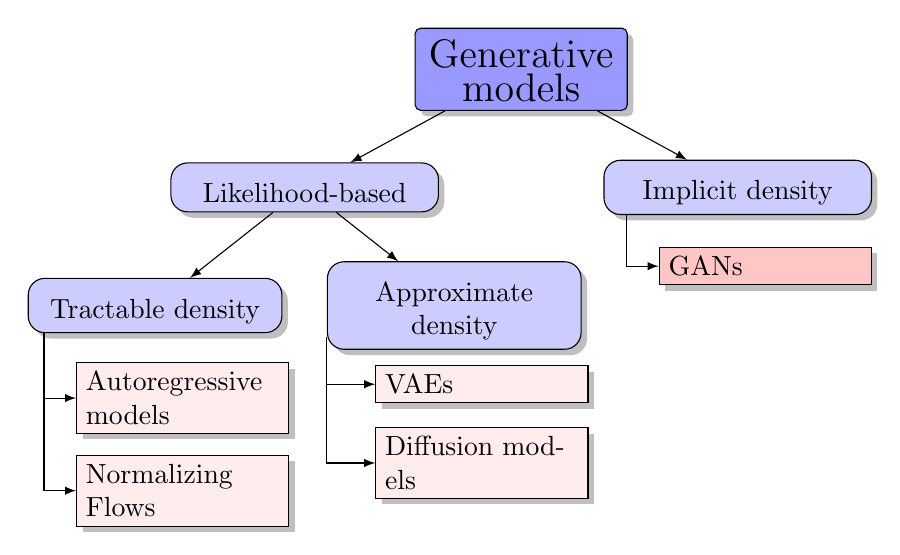
\begin{tikzpicture}[
	 	basic/.style  = {draw, text width=2cm, drop shadow, rectangle},
	 	root/.style   = {basic, rounded corners=2pt, thin, text height=1.1em, text width=7em, align=center, fill=blue!40},
	 	level 1/.style={sibling distance=55mm},
	 	level 2/.style = {basic, rounded corners=6pt, thin, align=center, fill=blue!20, text height=1.1em, text width=9em, sibling distance=38mm},
	 	level 3/.style = {basic, rounded corners=6pt, thin,align=center, fill=blue!20, text width=8.5em},
	 	level 4/.style = {basic, thin, align=left, fill=pink!30, text width=7em},
	 	level 5/.style = {basic, thin, align=left, fill=pink!90, text width=7em},
		edge from parent/.style={->,draw},
		>=latex]
		
		% root of the the initial tree, level 1
		\node[root] {\Large Generative models}
		% The first level, as children of the initial tree
		child {node[level 2] (c1) {Likelihood-based}
			child {node[level 3] (c11) {Tractable density}}
			child {node[level 3] (c12) {Approximate density}}
		}
		child {node[level 2] (c2) {Implicit density}};
		
		% The second level, relatively positioned nodes
		\begin{scope}[every node/.style={level 4}]
		\node [below of = c11, yshift=-5pt, xshift=10pt] (c111) {Autoregressive models};
		\node [below of = c111, yshift=-5pt] (c112) {Normalizing Flows};
		
		\node [below of = c12, xshift=10pt] (c121) {VAEs};
		\node [below of = c121] (c122) {Diffusion models};
		
		\end{scope}
		
		% The second level, relatively positioned nodes
		\begin{scope}[every node/.style={level 5}]
		\node [below of = c2, xshift=10pt] (c21) {GANs};
		\end{scope}
		
		
		% lines from each level 1 node to every one of its "children"
		\foreach \value in {1,2}
		\draw[->] (c11.194) |- (c11\value.west);
		
		\foreach \value in {1,2}
		\draw[->] (c12.194) |- (c12\value.west);
		
		\draw[->] (c2.194) |- (c21.west);
		
	\end{tikzpicture}
\end{frame}
%=======
\begin{frame}{Likelihood based models}
	Is likelihood a good measure of model quality?
	\begin{minipage}[t]{0.48\columnwidth}
		\begin{block}{Poor likelihood \\ Great samples}
			\vspace{-0.3cm}
			\[
				p_1(\bx) = \frac{1}{n} \sum_{i=1}^n \cN(\bx | \bx_i, \epsilon \bI)
			\]
			For small $\epsilon$ this model will generate samples with great quality, but likelihood will be very poor.
		\end{block}
	\end{minipage}%
	\begin{minipage}[t]{0.52\columnwidth}
		\begin{block}{Great likelihood \\ Poor samples}
			\vspace{-0.3cm}
			\[
				p_2(\bx) = 0.01p(\bx) + 0.99p_{\text{noise}}(\bx)
			\]
			\begin{multline*}
				\log \left[ 0.01p(\bx) + 0.99p_{\text{noise}}(\bx) \right] \geq  \\ \geq \log \left[ 0.01p(\bx) \right]  = \log p(\bx) - \log 100
			\end{multline*}
		Noisy irrelevant samples, but for high dimensions $\log p(\bx)$ becomes proportional to $m$.
		\end{block}
	\end{minipage}
	\myfootnotewithlink{https://arxiv.org/abs/1511.01844}{Theis L., Oord A., Bethge M. A note on the evaluation of generative models, 2015}
\end{frame}
%=======
\begin{frame}{Likelihood-free learning}
	\begin{itemize}
		\item Likelihood is not a perfect quality measure for generative model.
		\item Likelihood could be intractable.
	\end{itemize}
	\begin{block}{Where did we start}
	 We would like to approximate true data distribution $\pi(\bx)$.
		Instead of searching true $\pi(\bx)$ over all probability distributions, learn function approximation $p(\bx | \btheta) \approx \pi(\bx)$.
	\end{block}
	Imagine we have two sets of samples 
	\begin{itemize}
		\item $\cS_1 = \{\bx_i\}_{i=1}^{n_1} \sim \pi(\bx)$ -- real samples;
		\item $\cS_2 = \{\bx_i\}_{i=1}^{n_2} \sim p(\bx | \btheta)$ -- generated (or fake) samples.
	\end{itemize}
	\begin{block}{Two sample test}
		\vspace{-0.3cm}
		\[
			H_0: \pi(\bx) = p(\bx | \btheta), \quad H_1: \pi(\bx) \neq p(\bx | \btheta)
		\]
	\end{block}
	Define test statistic $T(\cS_1, \cS_2)$. The test statistic is likelihood free.
	If $T(\cS_1, \cS_2) < \alpha$, then accept $H_0$, else reject it.
\end{frame}
%=======
\begin{frame}{Likelihood-free learning}
	\begin{block}{Two sample test}
		\vspace{-0.5cm}
		\[
			H_0: \pi(\bx) = p(\bx | \btheta), \quad H_1: \pi(\bx) \neq p(\bx | \btheta)
		\]
		\vspace{-0.8cm}
	\end{block}
	\begin{block}{Desired behaviour}
		\begin{itemize}
			\item $p(\bx | \btheta)$ minimizes the value of test statistic~$T(\cS_1, \cS_2)$.
			\item It is hard to find an appropriate test statistic in high dimensions. $T(\cS_1, \cS_2)$ could be learnable.
		\end{itemize}
	\end{block}
	\vspace{-0.3cm}
	\begin{block}{GAN objective}
		\begin{itemize}
			\item \textbf{Generator:} generative model $\bx = G(\bz)$, which makes generated sample more realistic.
			\item \textbf{Discriminator:} a classifier $D(\bx) \in [0, 1]$, which distinguishes real samples from generated samples.
		\end{itemize}
		\[
			\min_{G} \max_D V(G, D) = \min_{G} \max_D \left[ \bbE_{\pi(\bx)} \log D(\bx) + \bbE_{p(\bz)} \log (1 - D(G(\bz))) \right]
		\]
	\end{block}
	 \myfootnotewithlink{https://arxiv.org/abs/1406.2661}{Goodfellow I. J. et al. Generative Adversarial Networks, 2014}
\end{frame}
%=======
\begin{frame}{Vanilla GAN optimality}
	\begin{block}{Theorem}
	The minimax game 
		\vspace{-0.1cm}
		\[
			\min_{G} \max_D V(G, D) = \min_{G} \max_D \left[ \bbE_{\pi(\bx)} \log D(\bx) + \bbE_{p(\bz)} \log (1 - D(G(\bz))) \right]
		\]
	has the global optimum $\pi(\bx) = p(\bx | \btheta)$, in this case $D^*(\bx) = 0.5$.
	\end{block}
	\begin{block}{Proof (fixed $G$)}
		\vspace{-0.5cm}
		\begin{align*}
			V(G, D) &= \bbE_{\pi(\bx)} \log D(\bx) + \bbE_{p(\bx | \btheta)} \log (1 - D(\bx)) \\
			&= \int \underbrace{\left[ \pi(\bx) \log D(\bx) + p(\bx | \btheta)\log (1 - D(\bx) \right]}_{y(D)} d \bx
		\end{align*}
		\vspace{-0.2cm}
		\[
			\frac{d y(D)}{d D} = \frac{\pi(\bx)}{D(\bx)} - \frac{p(\bx | \btheta)}{1 - D(\bx)} = 0 \quad \Rightarrow \quad D^*(\bx) = \frac{\pi(\bx)}{\pi(\bx) + p(\bx | \btheta)}
		\]
	\end{block}
	\myfootnotewithlink{https://arxiv.org/abs/1406.2661}{Goodfellow I. J. et al. Generative Adversarial Networks, 2014}
\end{frame}
%=======
\begin{frame}{Vanilla GAN optimality}
	\begin{block}{Proof continued (fixed $D = D^*$)}
		\vspace{-0.5cm}
		\begin{multline*}
			V(G, D^*) = \bbE_{\pi(\bx)} \log \frac{\pi(\bx)}{\pi(\bx) + p(\bx | \btheta)} + \bbE_{p(\bx | \btheta)} \log \frac{p(\bx | \btheta)}{\pi(\bx) + p(\bx | \btheta)} \\
		 = KL \left(\pi(\bx) || \frac{\pi(\bx) + p(\bx | \btheta)}{2}\right) + KL \left(p(\bx | \btheta) || \frac{\pi(\bx) + p(\bx | \btheta)}{2}\right) - 2\log 2 \\
		 = 2JSD(\pi(\bx) || p(\bx | \btheta)) - 2\log 2.
		\end{multline*}
	\end{block}
	\vspace{-0.3cm}
	\begin{block}{Jensen-Shannon divergence (symmetric KL divergence)}
		\vspace{-0.2cm}
		\footnotesize
		\[
			JSD(\pi(\bx) || p(\bx | \btheta)) = \frac{1}{2} \left[KL \left(\pi(\bx) || \frac{\pi(\bx) + p(\bx | \btheta)}{2}\right) + KL \left(p(\bx | \btheta) || \frac{\pi(\bx) + p(\bx | \btheta)}{2}\right) \right]
		\]
	\end{block}
	Could be used as a distance measure!
	\[
		V(G^*, D^*) = -2\log 2, \quad \pi(\bx) = p(\bx | \btheta).
	\]
	
	 \myfootnotewithlink{https://arxiv.org/abs/1406.2661}{Goodfellow I. J. et al. Generative Adversarial Networks, 2014}
\end{frame}
%=======
\begin{frame}{Vanilla GAN optimality}
	\begin{block}{Theorem}
		The minimax game 
		\vspace{-0.1cm}
		\[
			\min_{G} \max_D  V(G, D) = \min_{G} \max_D \left[ \bbE_{\pi(\bx)} \log D(\bx) + \bbE_{p(\bz)} \log (1 - D(G(\bz))) \right]
		\]
		has the global optimum $\pi(\bx) = p(\bx | \btheta)$, in this case $D^*(\bx) = 0.5$.
	\end{block}
	\vspace{-0.2cm}
	\begin{block}{Proof}
	for fixed $G$:
	\[
		D^*(\bx) = \frac{\pi(\bx)}{\pi(\bx) + p(\bx | \btheta)}
	\]
	\vspace{-0.5cm} \\
	for fixed $D = D^*$:
	\[
		\min_{G} V(G, D^*) = \min_{G} \left[ 2 JSD(\pi || p) - \log 4 \right] = -\log 4, \quad \pi(\bx) = p(\bx | \btheta).
	\]
	\vspace{-0.6cm}
	\end{block}
	If the generator could be any function and the discriminator is optimal at every step, then the generator is guaranteed to converge to the data distribution.
	 \myfootnotewithlink{https://arxiv.org/abs/1406.2661}{Goodfellow I. J. et al. Generative Adversarial Networks, 2014}
\end{frame}
%=======
\begin{frame}{Vanilla GAN}
	\begin{block}{Objective}
		\vspace{-0.4cm}
		\[
		\min_{G} \max_D V(G, D) = \min_{G} \max_D \left[ \bbE_{\pi(\bx)} \log D(\bx) + \bbE_{p(\bz)} \log (1 - D(G(\bz))) \right]
		\]
		\vspace{-0.4cm}
	\end{block}

	\begin{figure}
		\centering
		\includegraphics[width=1.0\linewidth]{figs/gan_1}
	\end{figure}
	\begin{itemize}
		\item Generator updates are made in parameter space.
		\item Discriminator is not optimal at every step.
		\item Generator and discriminator loss keeps oscillating during GAN training.
	\end{itemize}

	 \myfootnotewithlink{https://arxiv.org/abs/1406.2661}{Goodfellow I. J. et al. Generative Adversarial Networks, 2014}
\end{frame}
%=======
\begin{frame}{Vanishing gradients}
	\begin{block}{Objective}
		\vspace{-0.4cm}
		\[
		\min_{G} \max_D V(G, D) = \min_{G} \max_D \left[ \bbE_{\pi(\bx)} \log D(\bx) + \bbE_{p(\bz)} \log (1 - D(G(\bz))) \right]
		\]
		\vspace{-0.4cm}
	\end{block}
	Early in learning, $G$ is poor, $D$ can reject samples with high confidence. In this case, $\log (1 - D(G(\bz)))$ saturates.
	\begin{minipage}[t]{0.5\columnwidth}
		\begin{figure}
			\centering
			\includegraphics[width=0.9\linewidth]{figs/vanishing_gradients_1}
		\end{figure}
	\end{minipage}%
	\begin{minipage}[t]{0.5\columnwidth}
		\begin{figure}
			\centering
			\includegraphics[width=0.9\linewidth]{figs/vanishing_gradients_2}
		\end{figure}
	\end{minipage}
	\myfootnotewithlink{https://arxiv.org/abs/1701.04862}{Arjovsky M., Bottou L. Towards Principled Methods for Training Generative Adversarial Networks, 2017}
\end{frame}
%=======
\begin{frame}{Vanishing gradients}
	\begin{block}{Objective}
		\vspace{-0.4cm}
		\[
		\min_{G} \max_D V(G, D) = \min_{G} \max_D \left[ \bbE_{\pi(\bx)} \log D(\bx) + \bbE_{p(\bz)} \log (1 - D(G(\bz))) \right]
		\]
		\vspace{-0.4cm}
	\end{block}
	\begin{minipage}[t]{0.45\columnwidth}
		\begin{block}{Non-saturating GAN}
		\begin{itemize}
			\item Maximize $\log D(G(z))$ instead of minimizing $\log (1 - D(G(\bz)))$. \\
			\item Gradients are getting much stronger, but the training is unstable (with increasing mean and variance).
		\end{itemize}
		\end{block}
	\end{minipage}%
	\begin{minipage}[t]{0.55\columnwidth}
		\begin{figure}
			\centering
			\includegraphics[width=1.0\linewidth]{figs/vanishing_gradients_3}
		\end{figure}
	\end{minipage}
	\myfootnotewithlink{https://arxiv.org/abs/1701.04862}{Arjovsky M., Bottou L. Towards Principled Methods for Training Generative Adversarial Networks, 2017}
\end{frame}
%=======
\begin{frame}{Mode collapse}
	The phenomena where the generator of a GAN collapses to one or few distribution modes.
	\vspace{-0.15cm}
	\begin{figure}
		\centering
		\includegraphics[width=0.75\linewidth]{figs/mode_collapse_1}
	\end{figure}
	\vspace{-0.2cm}
	\begin{figure}
		\centering
		\includegraphics[width=1.0\linewidth]{figs/mode_collapse_3}
	\end{figure}
	Alternate architectures, adding regularization terms, injecting small noise
	perturbations and other millions bags and tricks are used to avoid the mode collapse.
	
	\myfootnote{\href{https://arxiv.org/abs/1406.2661}{Goodfellow I. J. et al. Generative Adversarial Networks, 2014} \\
	\href{https://arxiv.org/abs/1611.02163}{Metz L. et al. Unrolled Generative Adversarial Networks, 2016}}
\end{frame}
%=======
\begin{frame}{Jensen-Shannon vs Kullback-Leibler }
	\begin{block}{Mode covering vs mode seeking}
		\vspace{-0.2cm}
		\[
			KL(\pi || p) = \int \pi(\bx) \log \frac{\pi(\bx)}{p(\bx)}d\bx, \quad KL(p || \pi) = \int p(\bx) \log \frac{p(\bx)}{\pi(\bx)}d\bx
		\]
		\[
		JSD(\pi || p) = \frac{1}{2} \left[KL \left(\pi(\bx) || \frac{\pi(\bx) + p(\bx)}{2}\right) + KL \left(p(\bx) || \frac{\pi(\bx) + p(\bx)}{2}\right) \right]
		\]
		\vspace{-0.4cm}
		
	\begin{minipage}[t]{0.33\columnwidth}
		\begin{figure}
			\includegraphics[width=\linewidth]{figs/forward_KL}
		\end{figure}
	\end{minipage}%
	\begin{minipage}[t]{0.33\columnwidth}
			\begin{figure}
				\includegraphics[width=\linewidth]{figs/reverse_KL}
			\end{figure}
	\end{minipage}%
	\begin{minipage}[t]{0.33\columnwidth}
			\begin{figure}
				\includegraphics[width=\linewidth]{figs/JSD}
			\end{figure}
	\end{minipage}
	\vspace{-0.3cm}
	\end{block}
\end{frame}
%=======
\begin{frame}{Mode collapse: Deep Convolutional GAN}
	\begin{figure}
		\centering
		\includegraphics[width=\linewidth]{figs/mode_collapse_4}
	\end{figure}
	\myfootnotewithlink{https://arxiv.org/abs/1701.07875}{Arjovsky M., Chintala S., Bottou L. Wasserstein GAN, 2017}
\end{frame}
%=======
\begin{frame}{Summary}
	\begin{itemize}
		\item Likelihood is not a perfect criteria to measure quality of generative model.
		\vfill
		\item Adversarial learning suggests to solve minimax problem to match the distributions.
		\vfill
		\item Vanilla GAN tries to optimize Jensen-Shannon divergence (in theory).
		\vfill		
		\item Mode collapse and vanishing gradients are the two main problems of vanilla GAN.  Lots of tips and tricks has to be used to make the GAN training is stable and scalable.
		\vfill
		\item KL and JS divergences work poorly as model objective in the case of disjoint supports.
	\end{itemize}
\end{frame}
%=======
\end{document} 